\begin{definition}
	Mówimy, że zbiór punktów na płaszczyźnie jest w pozycji ogólnej, jeśli żadne trzy nie są współliniowe.
\end{definition}

\begin{theorem}[Happy Ending Problem; Esther Klein]
	W dowolnym zbiorze \(5\) punktów na płaszczyźnie w pozycji ogólnej pewne \(4\) tworzą czworokąt wypukły.
\end{theorem}
\begin{proof}
	Jeśli otoczka wypukła tych pięciu punktów ma \(5\) albo \(4\) punkty, to teza jest oczywista. Rozważmy sytuację, gdy otoczka wypukła jest trójkątem.
	\begin{center}
		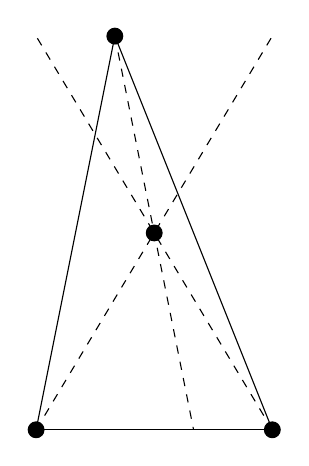
\begin{tikzpicture}
			\filldraw (0,0) circle (0.1);
			\filldraw (3,0) circle (0.1);
			\filldraw (1,5) circle (0.1);
			\filldraw (1.5,2.5) circle (0.1);
			\draw (0,0) -- (3,0);
			\draw (0,0) -- (1,5);
			\draw (3,0) -- (1,5);
			\draw[dashed] (0,0) -- (3,5);
			\draw[dashed] (3,0) -- (0,5);
			\draw[dashed] (1,5) -- (2,0);
		\end{tikzpicture}
	\end{center}
	Umieszczając piąty punkt w dowolnym z powstałych trójkątów otrzymujemy czworokąt wypukły powstały z punktu w środku trójkąta i odpowiednich wierzchołków trójkąta.
\end{proof}

\begin{theorem}[Erd\H{o}s-Szekeres; przez Happy Ending Problem]
	Dla dowolnego \(n\) istnieje takie \(N\), że jeśli \(N\) punktów na płaszczyźnie znajduje się w pozycji ogólnej to jakieś \(n\) z nich znajduje się w pozycji wypukłej.
\end{theorem}

\begin{proof}
	Na początek zauważmy, że jeśli dowolne \(4\) z \(n\) punktów w pozycji ogólnej tworzą czworokąt wypukły, to wszystkie \(n\) punktów tworzy wielokąt wypukły. Załóżmy nie wprost, że jakiś punkt leży we wnętrzu otoczki wypukłej takiego zbioru. Po striangulowaniu otoczki ten punkt leży w którymś z trójkątów. Czworokąt złożony z tego trójkąta i punktu w nim nie jest wypukły, a więc nie wszystkie czwórki są wypukłe -- sprzeczność.

	Niech \(N = R^{(4)}(2;n,5)\) i niech \(X\) będzie dowolny zbiorem \(N\) punktów w pozycji ogólnej. Definiujemy kolorowanie \(c:\binom{X}{4}\to [2]\) zadanie przez \(c(Y) = \left\{\begin{array}{lr}
		1 & Y \text{ wypukły} \\
		2 & Y \text{ wklęsły}
	\end{array}\right.\).
	Teraz albo mamy zbiór \(n\) punktów, gdzie każda czwórka tworzy czworokąt wypukły (a więc całość tworzy wielokąt wypukły), albo \(5\) punktów, gdzie każda czwórka tworzy wielokąt wklęsły -- to jednak nie może zajść na mocy Happy Ending Problem.
\end{proof}

